\documentclass[border=4pt,12pt]{standalone}
% House style for redrawn exam diagrams (diagram-v4: 0.4pt lines, filled -latex arrows, fine dashes; stipple and hatching drawn as real dots/lines (no PDF/SVG patterns, so they render in every browser and at any scale); transparent background). Every figure \input's this.
\usepackage{amsmath,amssymb}
\usepackage{txfonts}
\usepackage{pdfrender,xcolor}
% \halo{text}: label on shading. The shading stops just around each letter's outline (a thin knock-out that follows the
% glyphs, like the papers' typesetting), never a box. Owner: "I don't want a box around the text".
\newcommand{\halo}[1]{\leavevmode\rlap{\pdfrender{TextRenderingMode=2,LineWidth=2.2pt,LineJoinStyle=1,StrokeColor=white,FillColor=white}#1}#1}
\usepackage{tikz,pgfplots}
\pgfplotsset{compat=1.18}
\usetikzlibrary{arrows.meta,calc,angles,quotes,patterns,patterns.meta,intersections,positioning,decorations.markings,shapes.geometric}
% Stipple and hatching are drawn as actual dots / lines clipped to the region (path picture), NOT as pattern fills:
% SVG <pattern> fills vanish or blur when browsers scale the image, so the owner could not see the shading.
% Each dot is a 0.72pt square (keeps SVGs small; reads as a dot at print size). Dots sit on one global staggered grid, so neighbouring regions line up.
\makeatletter
\newdimen\ex@x \newdimen\ex@y \newdimen\ex@xa \newdimen\ex@ya \newdimen\ex@xb \newdimen\ex@yb \newcount\ex@row
\def\exam@stipplecolor{black!75}\def\exam@dotr{0.42pt}\def\exam@dotgap{2.5}
\def\ex@rowdots{\ifdim\ex@x<\ex@xb \pgfpathrectangle{\pgfqpoint{\dimexpr\ex@x-0.36pt\relax}{\dimexpr\ex@y-0.36pt\relax}}{\pgfqpoint{0.72pt}{0.72pt}}\advance\ex@x by \exam@dotgap pt\relax\expandafter\ex@rowdots\fi}
\def\exam@stipple{%
  \pgftransformreset% dots are sized in real points even inside scaled pictures
  \pgfpointanchor{path picture bounding box}{south west}\ex@xa=\pgf@x \ex@ya=\pgf@y
  \pgfpointanchor{path picture bounding box}{north east}\ex@xb=\pgf@x \ex@yb=\pgf@y
  \pgfsetfillcolor{\exam@stipplecolor}\pgfmathsetmacro\ex@h{\exam@dotgap/2}%
  \pgfmathtruncatemacro\ex@r{floor(\ex@ya/\ex@h)-1}\ex@row=\ex@r\relax
  \ex@y=\ex@r\dimexpr\ex@h pt\relax
  \loop\ifdim\ex@y<\ex@yb
    \pgfmathtruncatemacro\ex@c{floor(\ex@xa/\exam@dotgap)-1}\ex@x=\ex@c\dimexpr\exam@dotgap pt\relax
    \ifodd\ex@row \advance\ex@x by \ex@h pt\fi
    \ex@rowdots
    \advance\ex@y by \ex@h pt \advance\ex@row by 1
    \ifnum\numexpr\ex@row-(\ex@row/4)*4\relax=0 \pgfusepath{fill}\fi% flush every 4 rows: bounded TeX memory, few clip copies in the SVG
  \repeat\pgfusepath{fill}}
\newdimen\ex@d
\def\exam@hatch#1{% #1 = 1 for /, -1 for \ ; lines 45 degrees, 3pt apart
  \pgftransformreset
  \pgfpointanchor{path picture bounding box}{south west}\ex@xa=\pgf@x \ex@ya=\pgf@y
  \pgfpointanchor{path picture bounding box}{north east}\ex@xb=\pgf@x \ex@yb=\pgf@y
  \ex@d=\dimexpr\ex@yb-\ex@ya\relax \ex@x=\dimexpr\ex@xa-\ex@d\relax
  \loop\ifdim\ex@x<\ex@xb
    \ifnum#1>0 \pgfpathmoveto{\pgfqpoint{\ex@x}{\ex@ya}}\pgfpathlineto{\pgfqpoint{\dimexpr\ex@x+\ex@d\relax}{\ex@yb}}%
    \else \pgfpathmoveto{\pgfqpoint{\ex@x}{\ex@yb}}\pgfpathlineto{\pgfqpoint{\dimexpr\ex@x+\ex@d\relax}{\ex@ya}}\fi
    \advance\ex@x by 4.24pt
  \repeat
  \pgfsetlinewidth{0.4pt}\pgfsetstrokecolor{black}\pgfusepath{stroke}}
\def\examstipple{\exam@stipple}\def\examhatch{\exam@hatch}\def\examsetstipplecolor#1{\def\exam@stipplecolor{#1}}\def\examsetdotgap#1{\def\exam@dotgap{#1}}
\makeatother
% (legacy pattern kept for old files)
% staggered stipple like the NESA papers' dotted shading
\pgfdeclarepatternformonly{exam stipple}{\pgfpointorigin}{\pgfqpoint{2.2pt}{2.2pt}}{\pgfqpoint{2.2pt}{2.2pt}}{%
  \pgfpathcircle{\pgfqpoint{0.55pt}{0.55pt}}{0.42pt}\pgfpathcircle{\pgfqpoint{1.65pt}{1.65pt}}{0.42pt}\pgfusepath{fill}}
\tikzset{
  every picture/.style={line width=0.6pt, >={Latex[length=2mm,width=1.3mm]}},
  curve/.style={line width=0.6pt},
  open arrow/.style={-{Latex[length=2mm,width=1.3mm]}},  % owner: filled -latex heads everywhere, no open chevrons
  aux/.style={dash pattern=on 2pt off 1.5pt, line width=0.6pt},
  shade/.code={\def\exA{#1}\def\exB{none}\ifx\exA\exB\else\pgfkeysalso{fill=black!18}\fi},
  shade/.default=on,
  shade dots/.style={fill=none, path picture={\examstipple}},
  stipple color/.code={\examsetstipplecolor{#1}},
  stipple gap/.code={\examsetdotgap{#1}},
  shade dense dots/.style={fill=none, stipple gap=1.6, path picture={\examstipple}},
  shade hatch/.style={fill=none, path picture={\examhatch{1}}},
  shade hatch reverse/.style={fill=none, path picture={\examhatch{-1}}},
  shade solid/.style={fill=black},
  pt/.style={circle, fill, inner sep=1.1pt},
  open pt/.style={circle, draw, fill=white, inner sep=1.1pt},
}
\pgfplotsset{
  exam axes/.style={axis lines=middle, axis line style={->}, xlabel={$x$}, ylabel={$y$},
    xlabel style={anchor=west}, ylabel style={anchor=south}, tick label style={font=\small},
    every axis plot/.append style={line width=0.6pt, black}, samples=200, clip=false,
    enlargelimits=false, axis on top},
}

\begin{document}
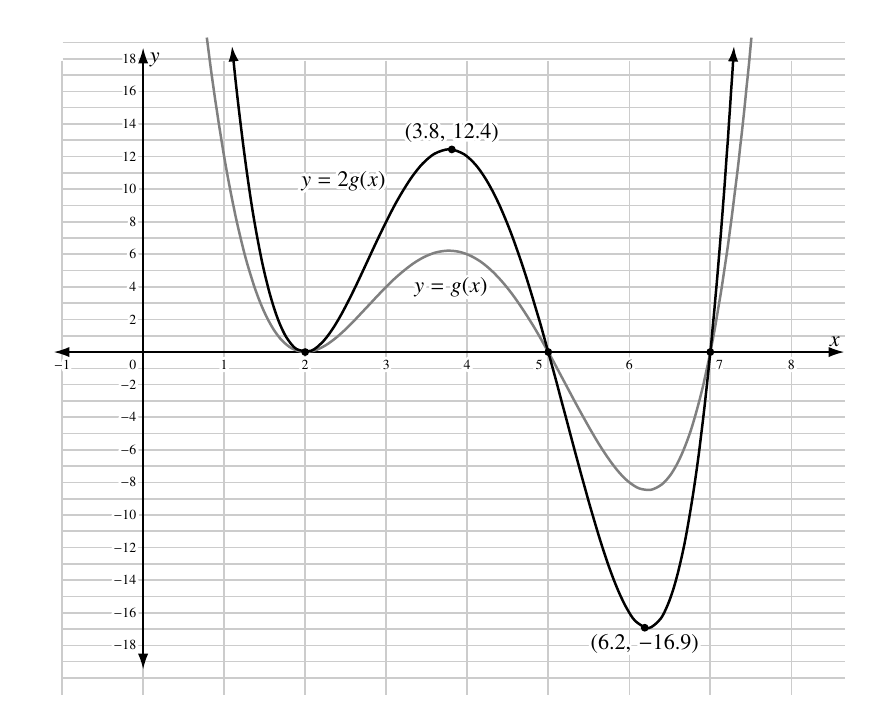
\begin{tikzpicture}[x=0.0127cm, y=-0.0127cm]
  \begin{scope}
  \clip (0,0) rectangle (818,668);
  \draw[black!20] (34.4,33) -- (34.4,668);
  \draw[black!20] (115.5,33) -- (115.5,668);
  \draw[black!20] (196.6,33) -- (196.6,668);
  \draw[black!20] (277.6,33) -- (277.6,668);
  \draw[black!20] (358.7,33) -- (358.7,668);
  \draw[black!20] (439.7,33) -- (439.7,668);
  \draw[black!20] (520.8,33) -- (520.8,668);
  \draw[black!20] (601.9,33) -- (601.9,668);
  \draw[black!20] (682.9,33) -- (682.9,668);
  \draw[black!20] (764.0,33) -- (764.0,668);
  \draw[black!20] (35,650.5) -- (818,650.5);
  \draw[black!20] (35,634.2) -- (818,634.2);
  \draw[black!20] (35,617.9) -- (818,617.9);
  \draw[black!20] (35,601.6) -- (818,601.6);
  \draw[black!20] (35,585.3) -- (818,585.3);
  \draw[black!20] (35,569.0) -- (818,569.0);
  \draw[black!20] (35,552.7) -- (818,552.7);
  \draw[black!20] (35,536.4) -- (818,536.4);
  \draw[black!20] (35,520.1) -- (818,520.1);
  \draw[black!20] (35,503.8) -- (818,503.8);
  \draw[black!20] (35,487.5) -- (818,487.5);
  \draw[black!20] (35,471.2) -- (818,471.2);
  \draw[black!20] (35,454.9) -- (818,454.9);
  \draw[black!20] (35,438.6) -- (818,438.6);
  \draw[black!20] (35,422.3) -- (818,422.3);
  \draw[black!20] (35,406.0) -- (818,406.0);
  \draw[black!20] (35,389.7) -- (818,389.7);
  \draw[black!20] (35,373.4) -- (818,373.4);
  \draw[black!20] (35,357.1) -- (818,357.1);
  \draw[black!20] (35,340.8) -- (818,340.8);
  \draw[black!20] (35,308.2) -- (818,308.2);
  \draw[black!20] (35,291.9) -- (818,291.9);
  \draw[black!20] (35,275.6) -- (818,275.6);
  \draw[black!20] (35,259.3) -- (818,259.3);
  \draw[black!20] (35,243.0) -- (818,243.0);
  \draw[black!20] (35,226.7) -- (818,226.7);
  \draw[black!20] (35,210.4) -- (818,210.4);
  \draw[black!20] (35,194.1) -- (818,194.1);
  \draw[black!20] (35,177.8) -- (818,177.8);
  \draw[black!20] (35,161.5) -- (818,161.5);
  \draw[black!20] (35,145.2) -- (818,145.2);
  \draw[black!20] (35,128.9) -- (818,128.9);
  \draw[black!20] (35,112.6) -- (818,112.6);
  \draw[black!20] (35,96.3) -- (818,96.3);
  \draw[black!20] (35,80.0) -- (818,80.0);
  \draw[black!20] (35,63.7) -- (818,63.7);
  \draw[black!20] (35,47.4) -- (818,47.4);
  \draw[black!20] (35,31.1) -- (818,31.1);
  \draw[black!20] (35,14.8) -- (818,14.8);
  \draw[black!20] (0,-1.5) -- (818,-1.5);
  \draw[<->] (26,324.5) -- (817,324.5);
  \draw[<->] (115.5,642) -- (115.5,20);
  \draw[smooth, black!50, line width=0.9pt] plot coordinates {(179.2,9.9) (180.8,22.1) (182.3,33.9) (183.9,46.0) (185.6,58.0) (187.3,70.1) (189.1,81.9) (190.9,94.0) (192.8,105.9) (194.7,117.8) (196.7,129.8) (198.8,141.7) (201.0,153.7) (203.3,165.6) (205.7,177.5) (208.1,189.2) (210.8,201.1) (213.6,212.9) (216.5,224.6) (219.7,236.3) (223.2,247.9) (226.9,259.5) (231.0,270.8) (235.6,282.0) (240.9,293.0) (247.0,303.4) (254.4,312.9) (263.8,320.6) (275.2,324.4) (287.1,322.9) (298.0,317.8) (307.9,310.7) (317.0,302.7) (325.6,294.2) (333.9,285.4) (342.2,276.6) (350.5,267.7) (358.9,259.1) (367.6,250.6) (376.8,242.7) (386.5,235.4) (396.9,229.3) (408.2,224.9) (420.1,223.1) (432.1,224.3) (443.5,228.4) (453.9,234.6) (463.3,242.3) (471.8,250.9) (479.7,260.1) (487.0,269.7) (493.9,279.7) (500.5,289.8) (506.9,300.1) (513.0,310.6) (518.9,321.2) (524.8,331.7) (530.5,342.4) (536.2,353.1) (541.9,363.8) (547.6,374.5) (553.4,385.1) (559.3,395.7) (565.3,406.2) (571.5,416.6) (578.1,426.8) (585.1,436.7) (592.7,446.1) (601.4,454.5) (611.7,460.9) (623.5,462.3) (634.3,457.0) (642.5,448.2) (648.9,437.9) (654.2,427.0) (658.8,415.8) (662.9,404.4) (666.5,392.8) (669.8,381.1) (672.9,369.5) (675.8,357.7) (678.4,345.9) (681.0,334.0) (683.4,322.1) (685.7,310.3) (687.9,298.3) (689.9,286.4) (691.9,274.5) (693.9,262.5) (695.7,250.6) (697.5,238.5) (699.3,226.5) (701.0,214.5) (702.6,202.5) (704.2,190.5) (705.7,178.6) (707.2,166.5) (708.7,154.5) (710.2,142.4) (711.6,130.3) (712.9,118.3) (714.3,106.3) (715.6,94.4) (716.9,82.2) (718.1,70.2) (719.3,58.1) (720.6,46.0) (721.8,34.0) (722.9,21.9) (724.0,10.0)};
  \draw[smooth, <->, line width=0.9pt] plot coordinates {(204.4,18.0) (206.0,33.7) (207.6,49.3) (209.3,64.8) (211.1,80.4) (213.0,96.1) (214.9,111.6) (216.9,127.1) (219.0,142.7) (221.2,158.2) (223.5,173.7) (226.0,189.2) (228.7,204.6) (231.6,220.0) (234.7,235.4) (238.2,250.6) (242.1,265.8) (246.6,280.9) (251.9,295.6) (258.8,309.7) (268.9,321.5) (283.7,323.2) (295.9,313.5) (305.3,301.0) (313.4,287.5) (320.7,273.7) (327.7,259.6) (334.4,245.4) (341.0,231.2) (347.6,217.0) (354.4,202.8) (361.3,188.8) (368.6,174.9) (376.5,161.4) (385.1,148.3) (395.0,136.1) (407.0,126.1) (421.8,121.6) (436.4,126.5) (448.0,137.0) (457.2,149.7) (465.0,163.3) (471.9,177.4) (478.1,191.8) (483.9,206.4) (489.2,221.1) (494.3,235.9) (499.2,250.9) (503.8,265.8) (508.3,280.8) (512.8,295.9) (517.0,311.0) (521.2,326.1) (525.4,341.2) (529.5,356.3) (533.5,371.5) (537.6,386.7) (541.6,401.8) (545.6,416.9) (549.7,432.1) (553.8,447.2) (558.0,462.3) (562.2,477.4) (566.6,492.4) (571.1,507.5) (575.8,522.4) (580.8,537.3) (586.2,552.0) (592.2,566.5) (599.1,580.5) (607.8,593.5) (621.1,600.7) (633.1,591.4) (640.3,577.4) (645.6,562.7) (649.9,547.6) (653.6,532.3) (656.9,517.1) (659.8,501.7) (662.5,486.1) (665.0,470.8) (667.4,455.1) (669.6,439.7) (671.7,424.1) (673.6,408.5) (675.5,393.0) (677.3,377.4) (679.0,361.8) (680.7,346.2) (682.3,330.7) (683.9,315.0) (685.3,299.5) (686.8,283.9) (688.2,268.1) (689.6,252.5) (690.9,237.0) (692.2,221.4) (693.5,205.6) (694.7,190.2) (695.9,174.4) (697.1,158.9) (698.2,143.3) (699.3,127.6) (700.5,111.9) (701.5,96.2) (702.6,80.5) (703.6,64.9) (704.7,49.2) (705.7,33.7) (706.6,18.1)};
  \node[anchor=north,inner sep=0,font=\tiny] at (34.4,331.5) {\halo{$-1$}};
  \node[anchor=north,inner sep=0,font=\tiny] at (196.6,331.5) {\halo{$1$}};
  \node[anchor=north,inner sep=0,font=\tiny] at (277.6,331.5) {\halo{$2$}};
  \node[anchor=north,inner sep=0,font=\tiny] at (358.7,331.5) {\halo{$3$}};
  \node[anchor=north,inner sep=0,font=\tiny] at (439.7,331.5) {\halo{$4$}};
  \node[anchor=north east,inner sep=0,font=\tiny] at (516,331.5) {\halo{$5$}};
  \node[anchor=north,inner sep=0,font=\tiny] at (601.9,331.5) {\halo{$6$}};
  \node[anchor=north west,inner sep=0,font=\tiny] at (688,331.5) {\halo{$7$}};
  \node[anchor=north,inner sep=0,font=\tiny] at (764.0,331.5) {\halo{$8$}};
  \node[anchor=north east,inner sep=0,font=\tiny] at (109.5,331.5) {\halo{$0$}};
  \node[anchor=east,inner sep=0,font=\tiny] at (109.5,617.9) {\halo{$-18$}};
  \node[anchor=east,inner sep=0,font=\tiny] at (109.5,585.3) {\halo{$-16$}};
  \node[anchor=east,inner sep=0,font=\tiny] at (109.5,552.7) {\halo{$-14$}};
  \node[anchor=east,inner sep=0,font=\tiny] at (109.5,520.1) {\halo{$-12$}};
  \node[anchor=east,inner sep=0,font=\tiny] at (109.5,487.5) {\halo{$-10$}};
  \node[anchor=east,inner sep=0,font=\tiny] at (109.5,454.9) {\halo{$-8$}};
  \node[anchor=east,inner sep=0,font=\tiny] at (109.5,422.3) {\halo{$-6$}};
  \node[anchor=east,inner sep=0,font=\tiny] at (109.5,389.7) {\halo{$-4$}};
  \node[anchor=east,inner sep=0,font=\tiny] at (109.5,357.1) {\halo{$-2$}};
  \node[anchor=east,inner sep=0,font=\tiny] at (109.5,291.9) {\halo{$2$}};
  \node[anchor=east,inner sep=0,font=\tiny] at (109.5,259.3) {\halo{$4$}};
  \node[anchor=east,inner sep=0,font=\tiny] at (109.5,226.7) {\halo{$6$}};
  \node[anchor=east,inner sep=0,font=\tiny] at (109.5,194.1) {\halo{$8$}};
  \node[anchor=east,inner sep=0,font=\tiny] at (109.5,161.5) {\halo{$10$}};
  \node[anchor=east,inner sep=0,font=\tiny] at (109.5,128.9) {\halo{$12$}};
  \node[anchor=east,inner sep=0,font=\tiny] at (109.5,96.3) {\halo{$14$}};
  \node[anchor=east,inner sep=0,font=\tiny] at (109.5,63.7) {\halo{$16$}};
  \node[anchor=east,inner sep=0,font=\tiny] at (109.5,31.1) {\halo{$18$}};
  \node[anchor=south,inner sep=0,font=\footnotesize] at (807.0,319.5) {$x$};
  \node[anchor=west,inner sep=0,font=\footnotesize] at (121.5,32.0) {$y$};
  \node[pt, inner sep=1pt] at (277.6,324.5) {};
  \node[pt, inner sep=1pt] at (520.8,324.5) {};
  \node[pt, inner sep=1pt] at (682.9,324.5) {};
  \node[pt, inner sep=1pt] at (424.3,121.8) {};
  \node[pt, inner sep=1pt] at (617.3,600.3) {};
  \node[anchor=south,inner sep=0,font=\footnotesize] at (424.3,115.6) {\halo{$(3.8,\,12.4)$}};
  \node[anchor=north,inner sep=0,font=\footnotesize] at (617.3,606.0) {\halo{$(6.2,\,-16.9)$}};
  \node[anchor=north,inner sep=0,font=\footnotesize] at (423.5,249.5) {\halo{$y=g(x)$}};
  \node[anchor=east,inner sep=0,font=\footnotesize] at (358.7,153.3) {\halo{$y=2g(x)$}};
  \end{scope}
\end{tikzpicture}
\end{document}
